\chapter{\texttt{biomarkeRs}: una aplicación web interactiva para detección de biomarcadores}

\section{Desarrollo de la aplicación}

Se ha realizado una aplicación interactiva que realiza el proceso descrito en el capítulo 4. Se ha utilizado para ello el paquete de R \textit{\texttt{\{Shiny\}}} (v.1.2.0) \cite{Chang2020}, que permite crear una interfaz que ejecuta código de R. La interfaz de usuario se ha mejorado mediante el uso de CSS. La aplicación desarrollada puede ejecutarse de forma local usando RStudio (un entorno de desarrollo integrado de R) \cite{RStudioTeam2020} y también está disponible de forma online en el enlace \url{https://dredondo.shinyapps.io/biomarkeRs/}.\\

El fichero \texttt{shiny\textbackslash app.R} del repositorio de GitHub asociado al trabajo \cite{Redondo-Sanchez2020} contiene el código de R desarrollado para crear la aplicación web.

\subsection{Características de las versiones web y local}

La versión web está alojada en \url{https://www.shinyapps.io/}, una plataforma de RStudio que permite la rápida integración de Shiny en una página web. La principal ventaja de esta versión es su accesibilidad mediante cualquier navegador, ya que no es necesaria ninguna instalación previa. Además, se puede acceder también desde cualquier dispositivo móvil sin pérdida de funcionalidades.\\

\begin{center}
	\textbf{Figura 42}. Imágenes de la aplicación ejecutándose en un iPhone 10.
\end{center}

\begin{figure}[H]
	\centering
	\begin{minipage}{.5\textwidth}
		\centering
	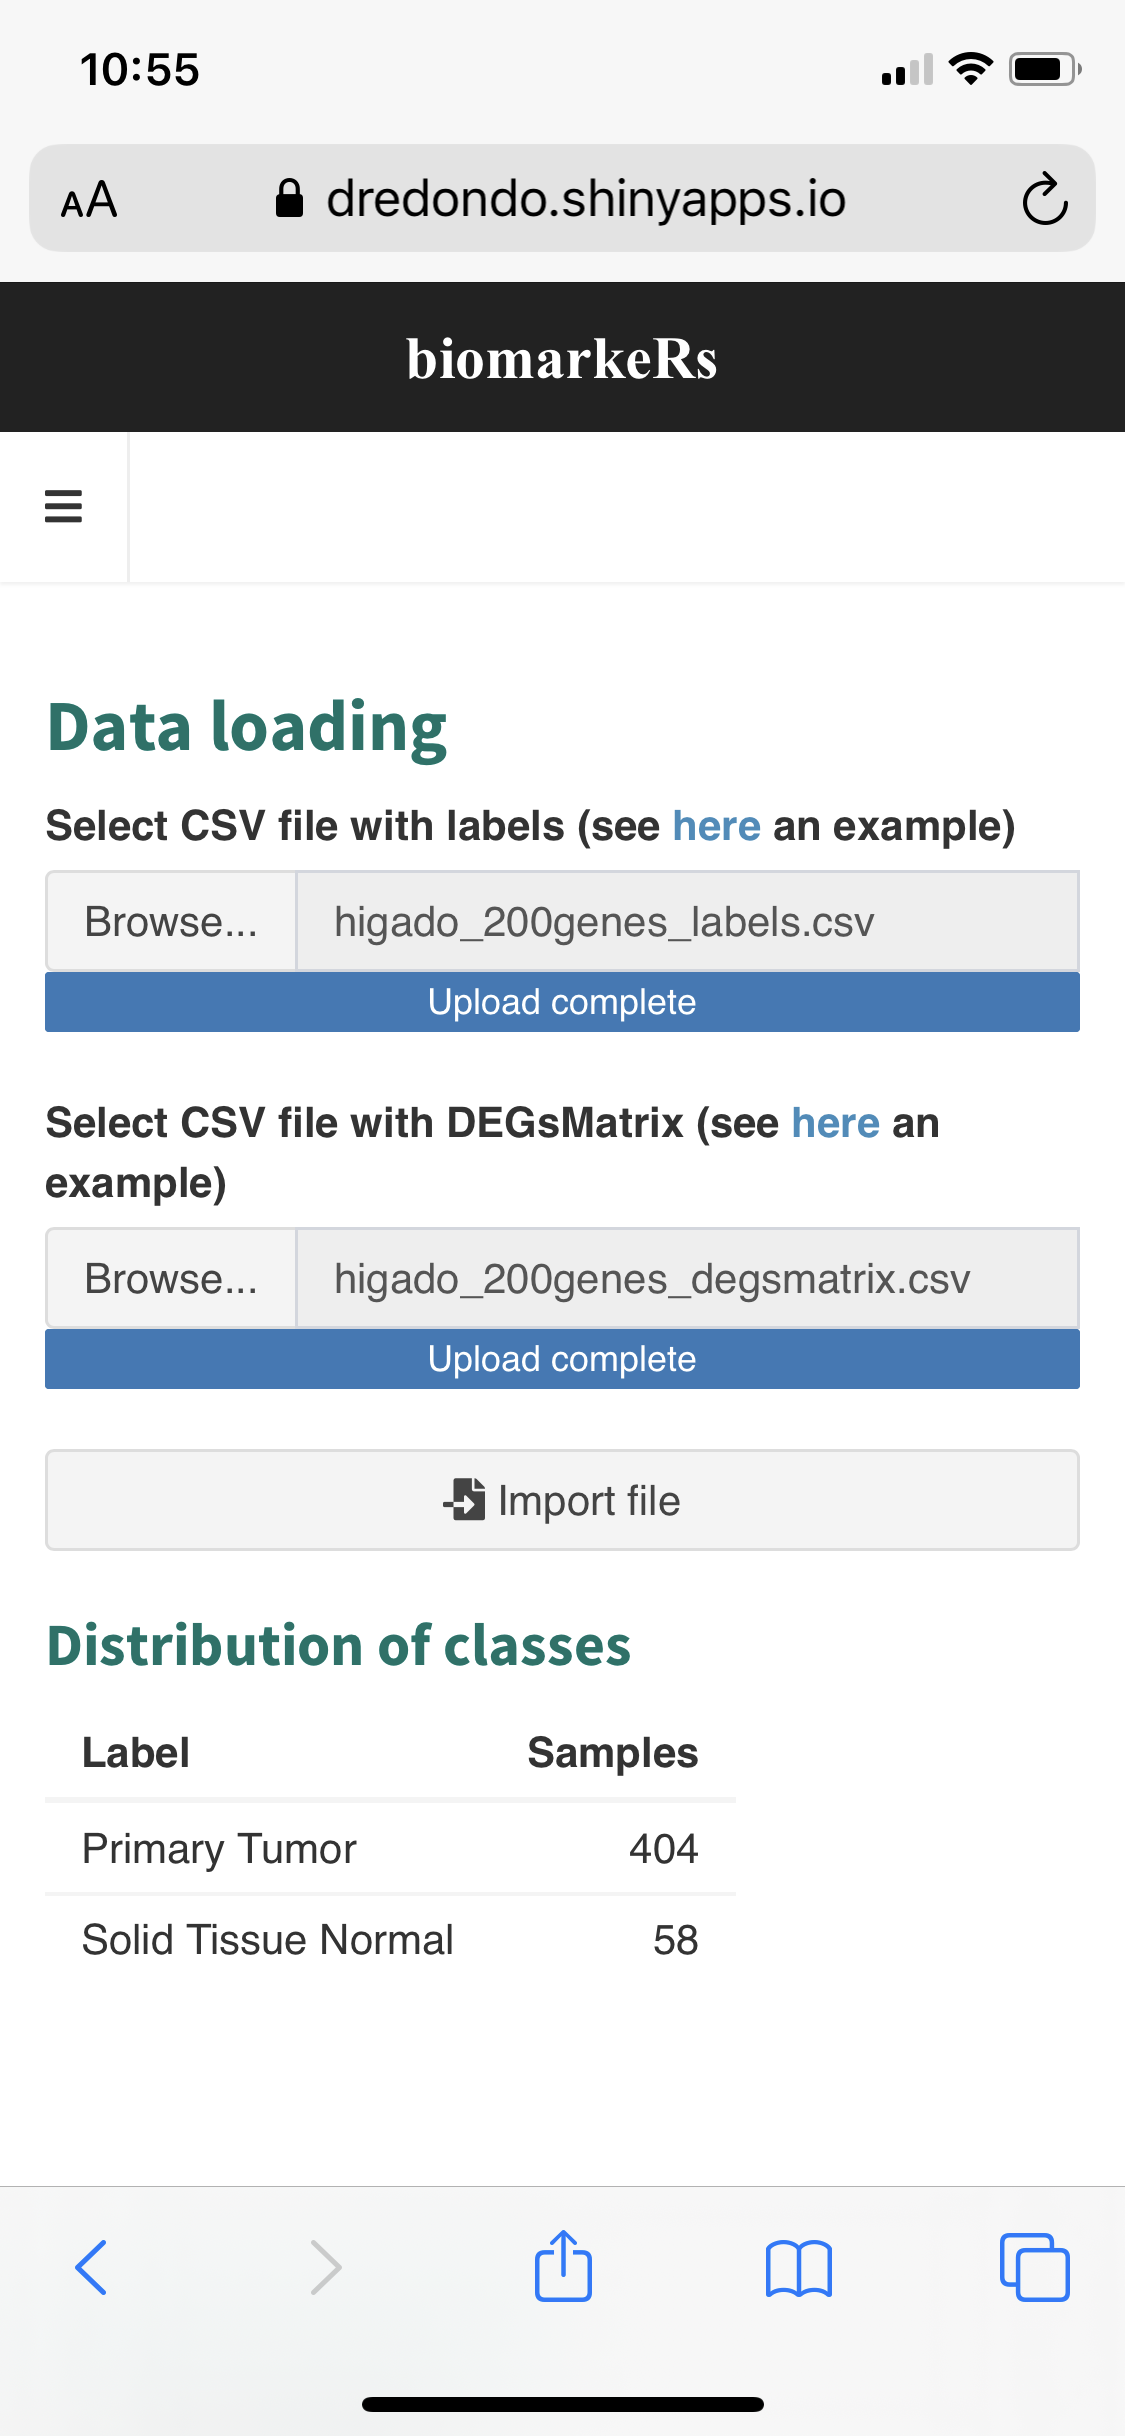
\includegraphics[width=.75\textwidth]{figuras/42_app_iphone1.png}
	\end{minipage}%
	\begin{minipage}{.5\textwidth}
		\centering
	 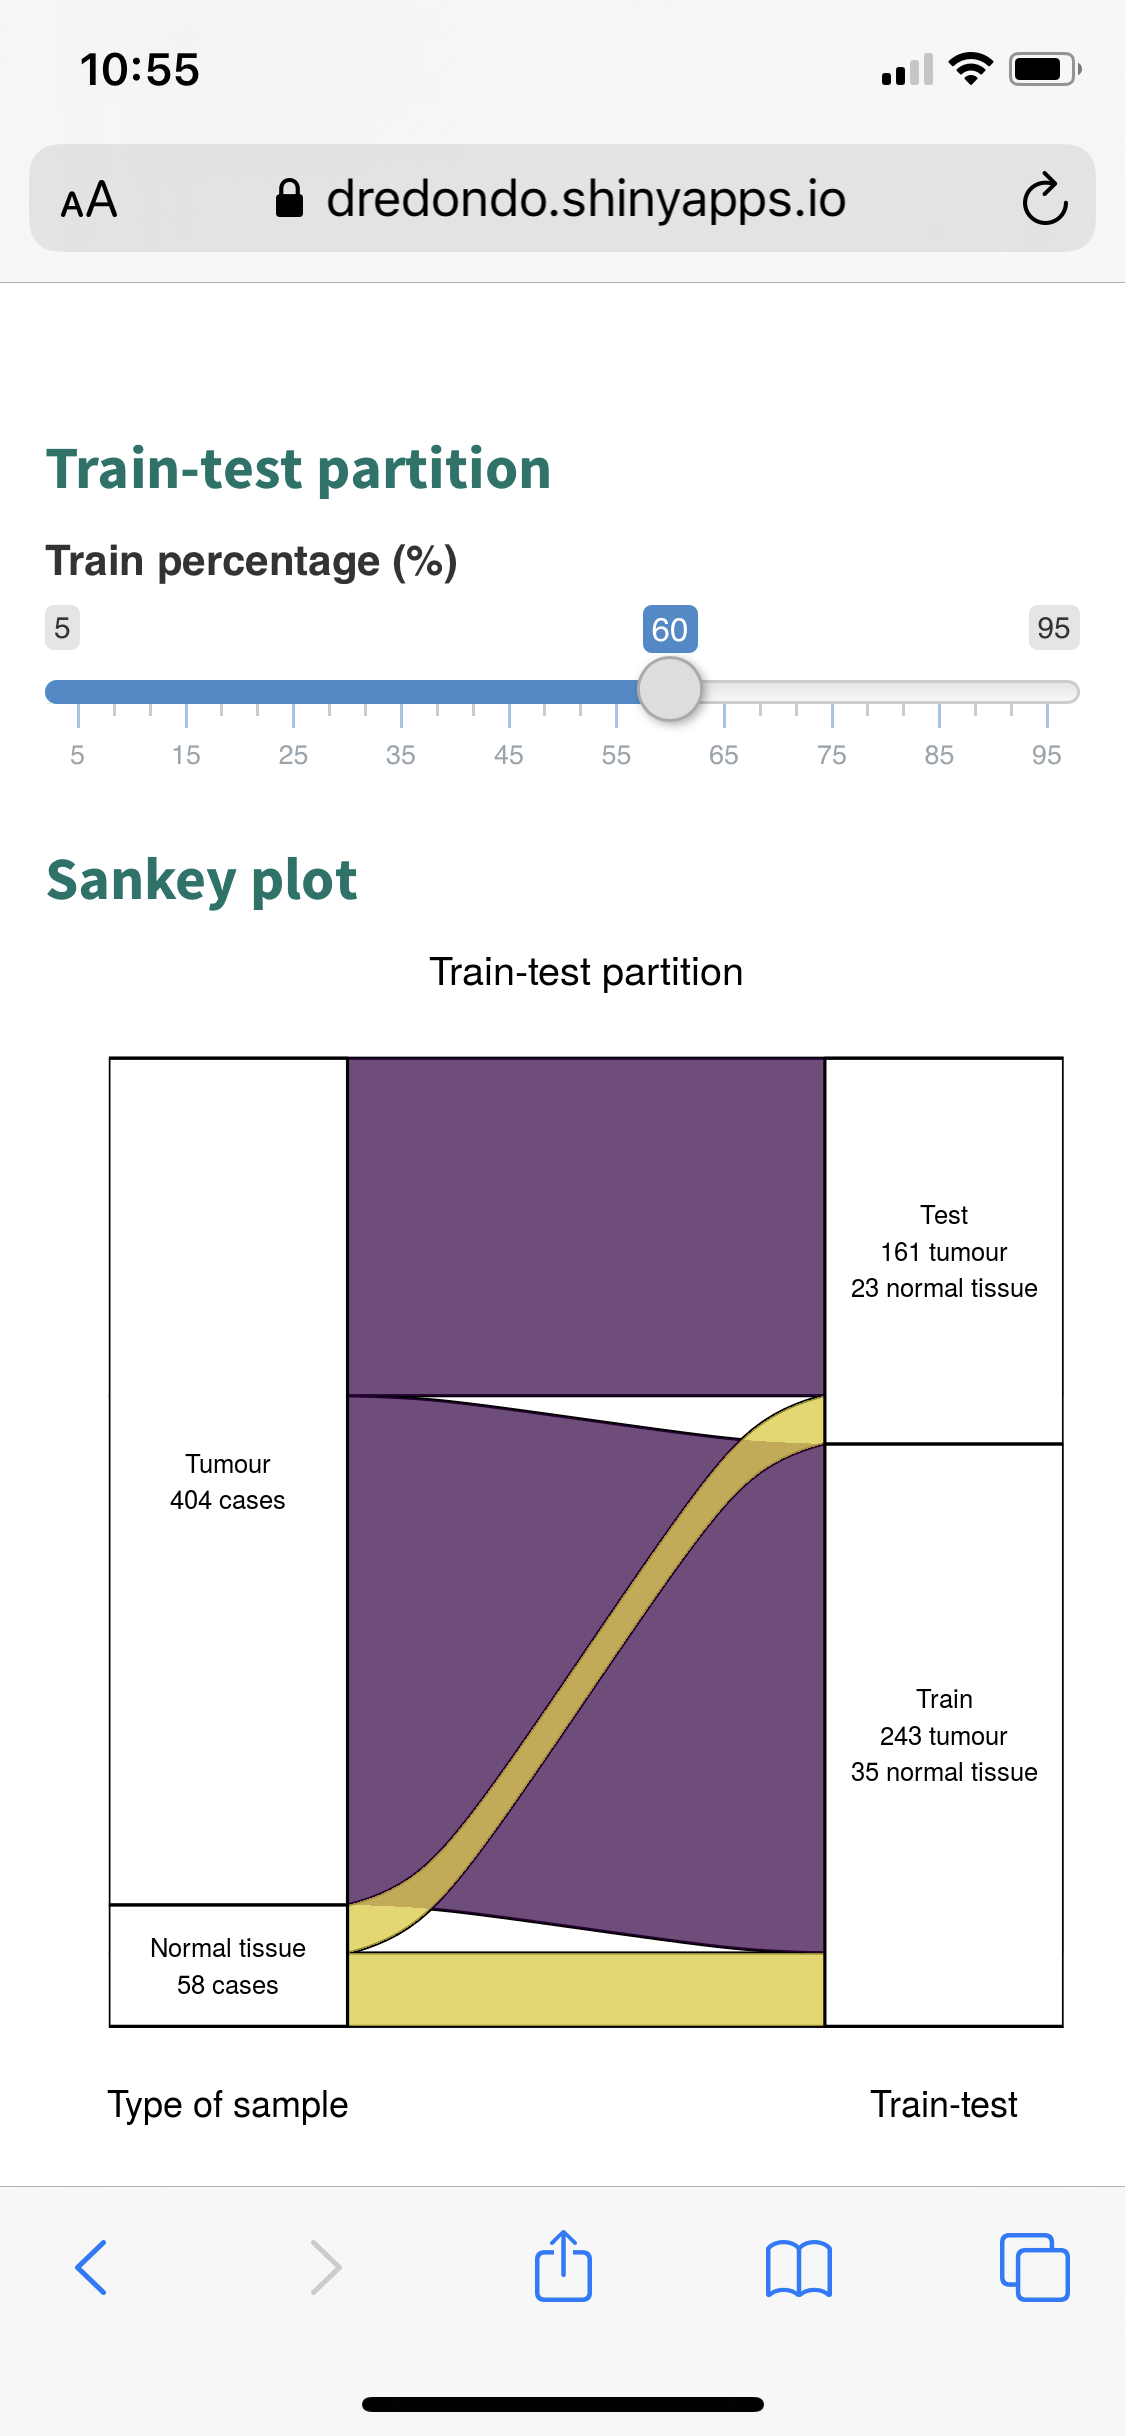
\includegraphics[width=.75\textwidth]{figuras/42_app_iphone2.png}
	\end{minipage}
\end{figure}

Para poder ejecutar la aplicación de forma local en un ordenador es necesario tener instalado una versión de R, de RStudio, y de todos los paquetes asociados a la aplicación. Además, puede haber problemas de compatibilidad entre los distintos paquetes. Este inconveniente no es tal en la versión web, gracias a que al realizar el despliegue a la web de la aplicación se realizan copias de las versiones de todos los paquetes que usa la aplicación Shiny localmente \cite{Shinyapps.ioteam2020}. De esta forma se asegura la estabilidad total de la versión web.\\

Uno de los aspectos en los que la versión local podría mejorar a la versión web es el coste computacional. La cuenta \textit{premium} de \url{https://www.shinyapps.io/} en la que está alojada la aplicación web permite hasta 8GB de RAM, característica que puede resultar insuficiente para el procesamiento de grandes cantidades de datos transcriptómicos. Otra posible limitación del tipo de cuenta es que ofrece un límite de 500 horas/mes de procesamiento. En el caso de alcanzar el límite, se podría mejorar el tipo de cuenta hasta alcanzar las 10.000 horas mensuales. Finalmente, la versión local es también mejor alternativa que la versión web cuando no hay conexión a internet o la conexión es lenta o inestable.

\section{Utilidades de la aplicación}


\textcolor{red}{por las limitaciones comentadas en el apartado anterior, fichero limitado a 200 genes para testear la aplicación web: DEGsExtraction con number = 200. Script reproducible para crear ficheros input}.\\

\textcolor{red}{Útil para realizar análisis genéticos para personas sin apenas conocimientos previos de programación. Capturas de pantalla con ejemplos. Escribir pequeño manual de uso. Quizá grabar vídeo mostrando la aplicación (y subir GIF a README del repositorio de GitHub).}